\documentclass[10pt,a4paper]{article}
\usepackage[margin=1.6cm]{geometry}
\usepackage{graphicx}
\usepackage{booktabs}
\usepackage{array}
\usepackage{tabularx}
\newcolumntype{L}[1]{>{\raggedright\arraybackslash}p{#1}}
\usepackage{enumitem}
\usepackage{xcolor}
\usepackage[hidelinks]{hyperref}

\setlist{noitemsep,topsep=2pt,leftmargin=*}
\setlength{\parindent}{0pt}
\setlength{\parskip}{4pt}

\title{Advanced Computer Architecture Project 1\\AlphaBot2 Multithreading and Multiprocessing Report}
\author{Names: \textit{Soham Dasare [4765654], Ka Wong Hui [4749653], Arjan Siddhpura [3707267]} \\Group Number: \textit{8} \quad Robot Number: \textit{11}}
\date{13 May 2026}

\begin{document}
\maketitle

\section{Project Objective}
The main goal of this project was to program the AlphaBot2 robot such that it could complete one round trip on the provided black track on the chart while executing three tasks that required concurrency: continuous line following, obstacle detection using infrared sensors with the correct number of buzzer signals, and camera-based object recognition with RGB LED feedback. The assignment required a parallel design because the robot must keep steering while also reacting to obstacles and recognizing a shoe, bottle, or mug, all at the same time.

\section{Hardware and Software Setup}
The implementation was developed for the AlphaBot2 platform with a Raspberry Pi 3B, DC motors, five infrared line sensors, left/right infrared obstacle sensors, a Pi camera, RGB LEDs, a buzzer, and servo support. The final project files with our implementation are \texttt{AlphaBot2v2.py} (v2 using multithreading) and \texttt{AlphaBot2v3.py} (v3 using multiprocessing). Object recognition used a quantized MobileNetV2 model from TorchVision with ImageNet labels to keep its resource footprint minimal. The target ImageNet classes were mapped to the required objects as follows: shoe classes to the red LED, bottle classes to yellow LEd, and mug/cup classes to green LED.

\begin{figure}[htbp]
    \centering
    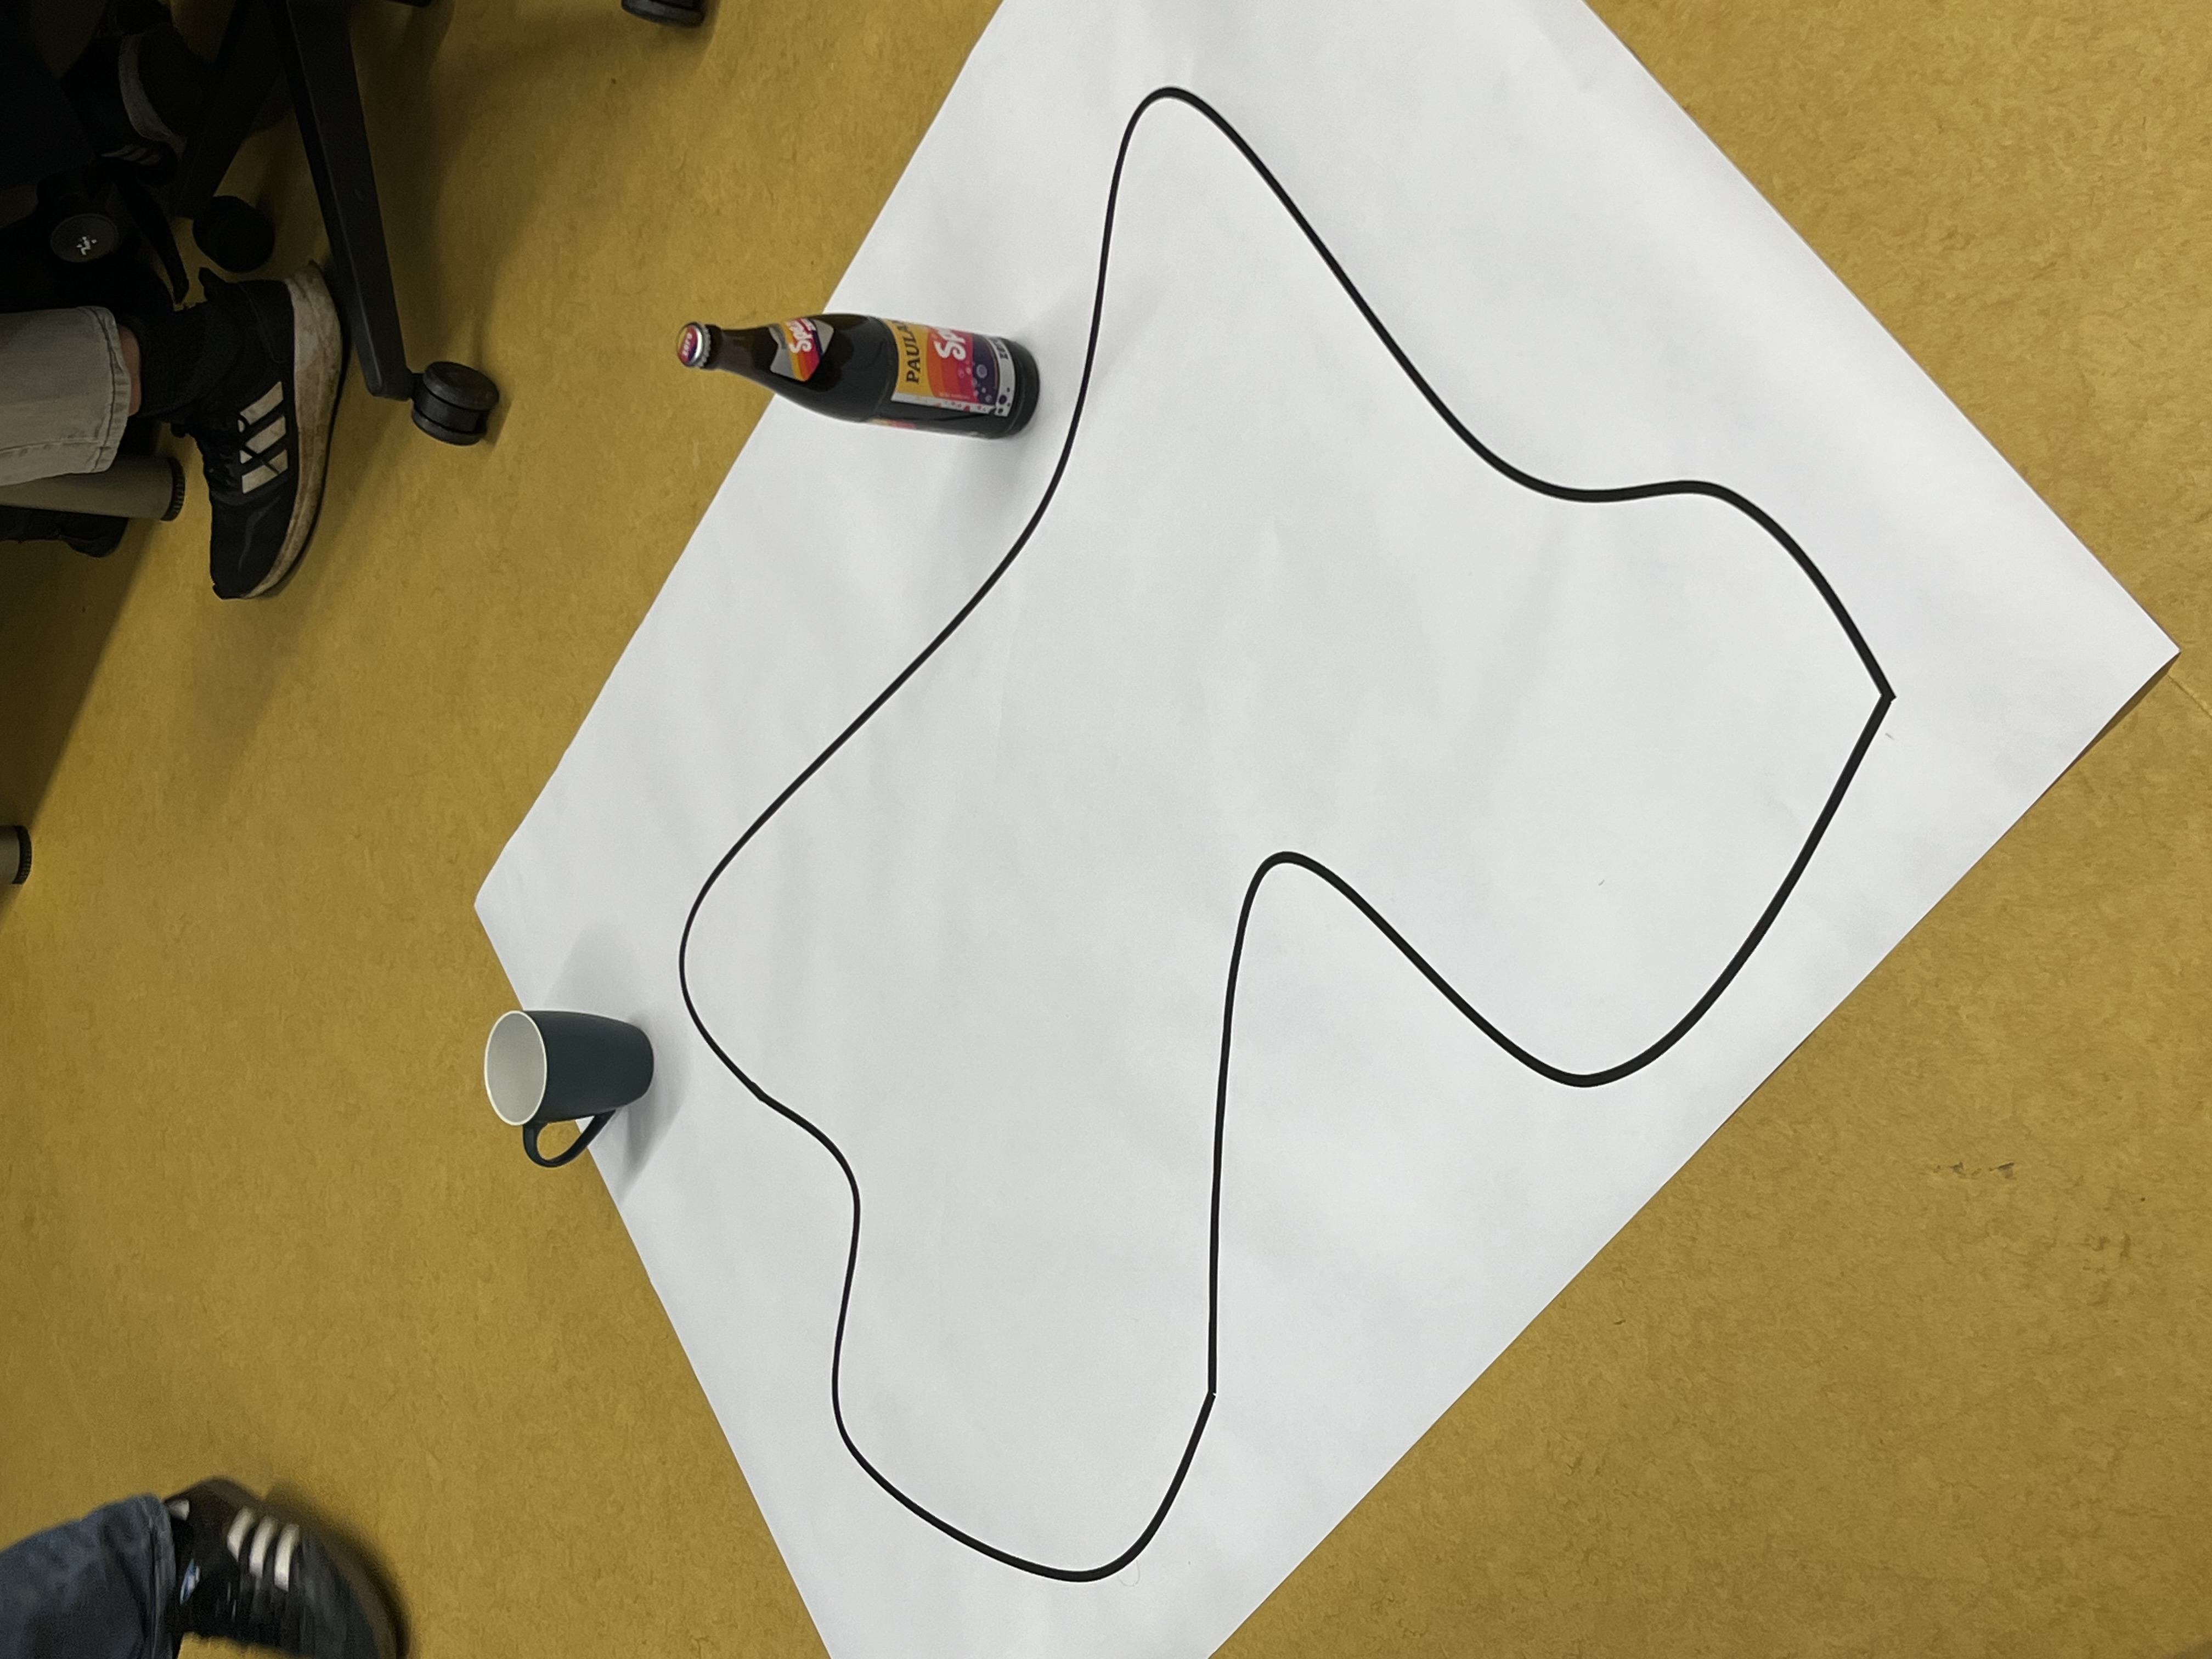
\includegraphics[width=0.58\linewidth,angle=-90]{media/IMG_2535.JPG}
    \caption{Reference track that we used for testing the AlphaBot2 line-following and object-response tasks.}
\end{figure}

\newpage
\section{Version 1: Sequential Baseline}
A purely sequential version would execute the same operations one after another: read line sensors and update motor PWM, poll obstacle sensors, perform buzzer delays, capture a camera frame, run neural-network inference, and update LEDs. This design is simple, but it causes missed control updates because camera inference and buzzer sleeps block the line-following loop, which would mean that the robot would often deviate from its original path. Moreover, the clock speed of the ARM Cortex-A53 processor on the Raspberry Pi 3B is 1.2 GHz, meaning each of the required tasks has around $\sim$200 million clock cycles ($\frac{1.2. \cdot 10^9}{6}$). In practice, we found this to show very poor performance near curves and hairpins, where the robot needs frequent sensor readings and motor corrections very quickly. Therefore, we had to separate time-critical motor control from slower perception and feedback tasks.

\section{Version 2: Multithreaded Design}
\texttt{AlphaBot2v2.py} implements the first concurrent solution using Python threads. A shared \texttt{threading.Event} acts as a stop signal, and a thread-safe \texttt{queue.Queue} transfers buzzer requests from obstacle detection to the buzzer worker.

\begin{table}[htbp]
\centering
\begin{tabular}{L{0.25\linewidth}L{0.27\linewidth}L{0.38\linewidth}}
\toprule
Task & Implementation & Responsibility \\
\midrule
Line following & \texttt{line\_following\_task} thread & Runs the fastest loop, reads calibrated reflectance sensors, computes steering correction, and drives the motors. \\
Obstacle detection & \texttt{obstacle\_detection\_task} thread & Polls left/right IR obstacle sensors, debounces detections for one second, and counts distinct objects. \\
Buzzer control & \texttt{beeper\_task} thread & Converts object count to one, two, or three short beeps without blocking detection or steering. \\
Object recognition & \texttt{object\_recognition\_task} thread & Captures camera frames, runs MobileNetV2 inference, and updates LED colors. \\
\bottomrule
\end{tabular}
\caption{Task distribution in our multithreaded implementation.}
\end{table}

For the line-following controller, we used fixed sensor limits \([210,193,218,184,247]\) and \([956,957,960,951,949]\), obtained from repeated calibration runs on the same printed track under the lab lighting. In practice, these values gave the most stable startup behaviour (less oscillation in the first seconds) and avoided run-to-run drift caused by quick recalibration before each demo run. The controller estimates the line position around a center value of 2000 and applies a proportional-derivative correction. The proportional term reacts to the current deviation from the centre of the line, while the derivative term reacts to how quickly the error is changing. We found this combination useful on the provided track because the route contains both long smooth sections and tight turns. The derivative term is normalized by elapsed time so that delayed samples do not create unstable steering spikes, which we also experienced before. We also added logic that detects sharp curves before the line is completely lost and performs a pivot turn if necessary. If no sensor sees the line, the robot enters a recovery mode and turns in the last known direction, reversing the recovery direction after a timeout to make sure it remains on the track.

We stored the calibration values were stored directly in the program after our testing using trial and error, instead of recalibrating at the start of every run. This made the demonstration more repeatable and deterministic because the robot could begin immediately with known minimum and maximum reflectance values for each of the five sensors. The values also compensate for small differences between individual sensors and for the contrast between the black tape and the surrounding paper. A fixed base speed was chosen to balance reliability and completion time: increasing speed reduced lap time, but made the robot more likely to overshoot the hairpin turns. Our testing also showed that it performed poorly if the width of the line altered by a lot.

Threading improves responsiveness because GPIO calls, camera capture, PyTorch native inference, and \texttt{sleep} calls release the Global Interpreter Lock (GIL) for significant parts of their runtime. However, the vision thread can still compete with the control loop during Python-level preprocessing and scheduling. This motivated the second version, where we implemented multiprocessing for true parallelism instead of just concurrency using multithreading.

\newpage
\section{Version 3: Multiprocessing Design}
\texttt{AlphaBot2v3.py} extends the design with multiprocessing. The main process owns the hardware that needs direct coordination, especially motor control, LEDs, camera capture, and cleanup. This is beacause there is only one set of resources shared among multiple processes. Separate processes handle CPU-intensive or independent tasks, while queues try to pass very compact messages (to minimize any latency spikes) between processes.

\begin{itemize}
    \item \textbf{Main process:} runs the highest-priority line-following loop, captures camera frames every approximately 0.2 seconds, resizes them to \(224\times224\) to quadratically minimize the amount of data to be sent, sends them to the vision process, receives LED commands, and performs safe shutdown. This is the main control manager process. 
    \item \textbf{Vision process:} initializes its own MobileNetV2 model, receives resized frames through \texttt{frame\_queue}, classifies objects, and sends color commands through \texttt{led\_queue}.
    \item \textbf{Obstacle process:} polls GPIO pins 16 and 19 for obstacle detection, debounces each new object, and sends the required beep count through \texttt{buzzer\_queue}.
    \item \textbf{Beeper thread:} remains a lightweight thread in the main process because it only toggles the buzzer GPIO and sleeps; this avoids blocking the line-following loop.
\end{itemize}

The multiprocessing version uses the \texttt{spawn} start method to avoid PyTorch/OpenMP deadlocks that can occur when forking after native thread pools have been initialized. The frame queue has size one, so that any stale camera frames are automatically avoided. This is important because robot actions should be based on the newest view of the environment, not on a backlog of old frames. Resizing frames before inter-process helped us reduce serialization overhead and keeps the main loop focused on steering the robot properly.

The design also follows a hardware-safety rule: the most direct actuator commands remain in the main process. The child processes do not attempt to drive the motors or write LED values directly. Instead, they send high-level commands such as ``set LEDs to yellow'' or ``beep twice'' to the main process. This reduces the chance of two processes writing conflicting GPIO states at the same time (i.e. race conditions) and makes shutdown simpler. During shutdown, the stop event is set, the buzzer thread is allowed to finish, the motors are stopped, the buzzer and LEDs are turned off, the camera server is stopped, and GPIO cleanup is called.

\section{Functional Behaviour}
In our testing, the final behaviour satisfied all the required demonstrations. First, the robot continuously followed the black track using calibrated line sensors and PD motor control. Second, obstacle detection counts distinct objects in front of the left or right IR sensors. A rising-edge check is used so that a single object is not counted repeatedly while it remains in front of the sensor. A one-second debounce interval further reduces false multiple counts caused by sensor noise or reflections. The first object triggers one beep, the second triggers two beeps, and the third triggers three beeps; we also used the modulo expression in the code to allow the sequence to repeat for any later detections.

Third, visual recognition maps detected objects to LED colors: shoe to red, bottle to yellow, and mug to green. The implementation checks ImageNet class IDs instead of only matching words in class names. This avoids any false positives, for example when a target word appears as part of an unrelated label. A confidence threshold is used so that any weak classifications do not immediately change the LED output. If no target object is recognized above the threshold, the LEDs are simply cleared.

\newpage
\section{System Configuration and Scheduling Experiments}
During testing we noticed that the Raspberry Pi 3B was not using all CPU cores. Even with the multithreaded and multiprocessing versions running, and even when the system was mostly idle, only one core appeared active. We tried to diagnose the problem and found out that the Raspberry Pi boot configuration required a change from \texttt{maxcpus=1} to \texttt{maxcpus=4} in \texttt{boot/firmware/cmdline.txt}, after which we rebooted the board. After this change, the operating system was able to schedule work across all four cores, making the multiprocessing design meaningful.

This was tested in the context of making all cores active and then running both the multithreaded and multiprogramming/multiprocessing approaches under the new configuration. In the multiprocessing version, the expected \texttt{htop} behaviour is three visibly active cores: the main process for line following and coordination, the vision process for PyTorch inference, and the obstacle process for IR polling. The beeper remains a thread in the main process because it only performs short GPIO writes and \texttt{sleep} calls.

We also considered whether different thread delays or Linux scheduling policies could improve navigation. Thread delays are useful to prevent tight resource heavy loops from saturating a CPU core, but they can also reduce control responsiveness if they are too long. Since object detection and camera recognition already introduce latency, increasing delays in the recognition or detection loops did not improve navigation significantly in our tests. However, Linux niceness or scheduling policy changes in the OS may help because they can give the line-following process higher priority than the slower perception tasks. This is especially relevant on the Raspberry Pi 3B, where CPU and memory bandwidth are quite limited.

The most useful delay experiment was therefore not to slow every task equally, but to keep the steering delay small and adjust only the non-critical tasks. For example, obstacle polling could tolerate a short delay because objects remain in the sensor range for more than one control cycle, and vision could slightly tolerate frame skipping because LED colour changes do not necessarily need millisecond timing. By contrast, the PD line-following loop must always remain frequent because each missed update increases the risk of overshooting a curve and derailing.

\begin{table}[htbp]
\centering
\small
\begin{tabularx}{\linewidth}{cX X}
\toprule
\# & Issue observed & Change applied \\
\midrule
1 & \texttt{fork()} with PyTorch/OpenMP could deadlock or pin child activity badly. & Used \texttt{mp.set\_start\_method('spawn')} so each child starts as a fresh interpreter. \\
2 & Main loop could saturate Core 0 at 100\%. & Added \texttt{time.sleep(0.01)} at the end of the main loop to yield CPU time. \\
3 & Sending full \(640\times480\) frames through \texttt{mp.Queue} was slow on the Pi 3B. & Resized frames to \(224\times224\) before \texttt{put\_nowait()}, reducing serialization overhead. \\
4 & Buzzer sleeps could block steering for up to several tenths of a second. & Moved buzzing into a dedicated \texttt{threading.Thread} using the same non-blocking pattern as v2. \\
\bottomrule
\end{tabularx}
\caption{Efficiency changes applied to the multiprocessing implementation.}
\end{table}

\newpage
\section{Results and Analysis}
Compared with a sequential design, both parallel versions reduce blocking in the control loop. In the sequential baseline, a full object-recognition cycle or a multi-beep buzzer sequence can delay steering updates long enough for the robot to drift from the line. The buzzer is a clear example: three beeps require several on/off delays, and these delays would be unacceptable if they occurred inside the steering loop. In the multithreaded version, these tasks run concurrently, so line following continues while the buzzer sounds and while the camera task processes frames. This greatly improved the stability and reduced the chance of missing sharp turns.

The multiprocessing version gave us the best architecture for this task. We found object recognition to be the most computationally expensive task, and moving it into a separate process prevented it from competing with the main control loop under the Python GIL. The obstacle process also polls independently at a short interval. As a result, the main process was able to maintain a consistent line-following period of about 10 ms while other processes handled perception and reactions. The performance improvement we saw was smoother track following, fewer missed obstacle events, and more reliable LED updates during camera inference.

The navigation itself is kept simple: it is based on a PD controller, following the standard PID-control principle that the proportional part corrects present error and the derivative part damps rapid error changes [\textit{\AA str\"om and H\"agglund, PID Controllers: Theory, Design and Tuning}]. We did not use an integral term because the robot does not need to remove a long-term steady-state offset; it needs fast local corrections while following a high-contrast black line. In this application, an integral term could also accumulate error during line loss and make recovery less stable. This was our reasoning.

Overall, we observed that both approaches worked, but for different reasons. Multithreading worked because many hardware and sleep operations release the GIL, making it a lightweight way to overlap the various tasks like line following, obstacle sensing, buzzing, and camera inference. Multiprocessing worked better after enabling all CPU cores because the expensive vision task could be offloaded on a separate core and communicate with the coordinator through queues. The parts that did not work well initially were related to system configuration and overhead: only one core was enabled, full-frame IPC between processes was quite slow, and unsafe direct hardware access from multiple processes would have created conflicts.

\begin{table}[htbp]
\centering
\begin{tabular}{L{0.22\linewidth}L{0.24\linewidth}L{0.30\linewidth}L{0.14\linewidth}}
\toprule
Implementation & Line stability & Object/LED response & Round-trip time \\
\midrule
Sequential baseline & Lowest; steering blocked by slow tasks & Delayed during motor updates or buzzer sleeps & \textit{~almost a minute but the robot did not properly finish its objectives, which is why measuring the timing was pointless} \\
Multithreading, v2 & Improved; steering runs concurrently & Good, but vision may still affect scheduling & \textit{~31.4 seconds} \\
Multiprocessing, v3 & Best; control separated from vision inference & Best; queues decouple perception and actions & \textit{~26.1 seconds} \\
\bottomrule
\end{tabular}
\caption{Performance comparison.}
\end{table}

\section{Conclusion}
From this project, we were able to learn that separating AlphaBot2 tasks was essential for reliable autonomous behaviour. The multithreaded version already improved responsiveness a lot by allowing the line following, obstacle detection, buzzing, and recognition to progress concurrently. The multiprocessing version was slightly stronger stronger because it isolated CPU-heavy vision inference from the motor-control loop and communicated through bounded queues using small, compressed messages. 

\end{document}